\documentclass{article}
\usepackage[utf8]{inputenc}
\usepackage{graphicx}

\title{Langkah-Langkah Membuat Aplikasi di APEX dengan Data Mahasiswa}
\author{Dyah Ayu Anandra }
\date{31 October 2019}

\begin{document}

\maketitle

\section{Login Oracle APEX Online}
\begin{center}
    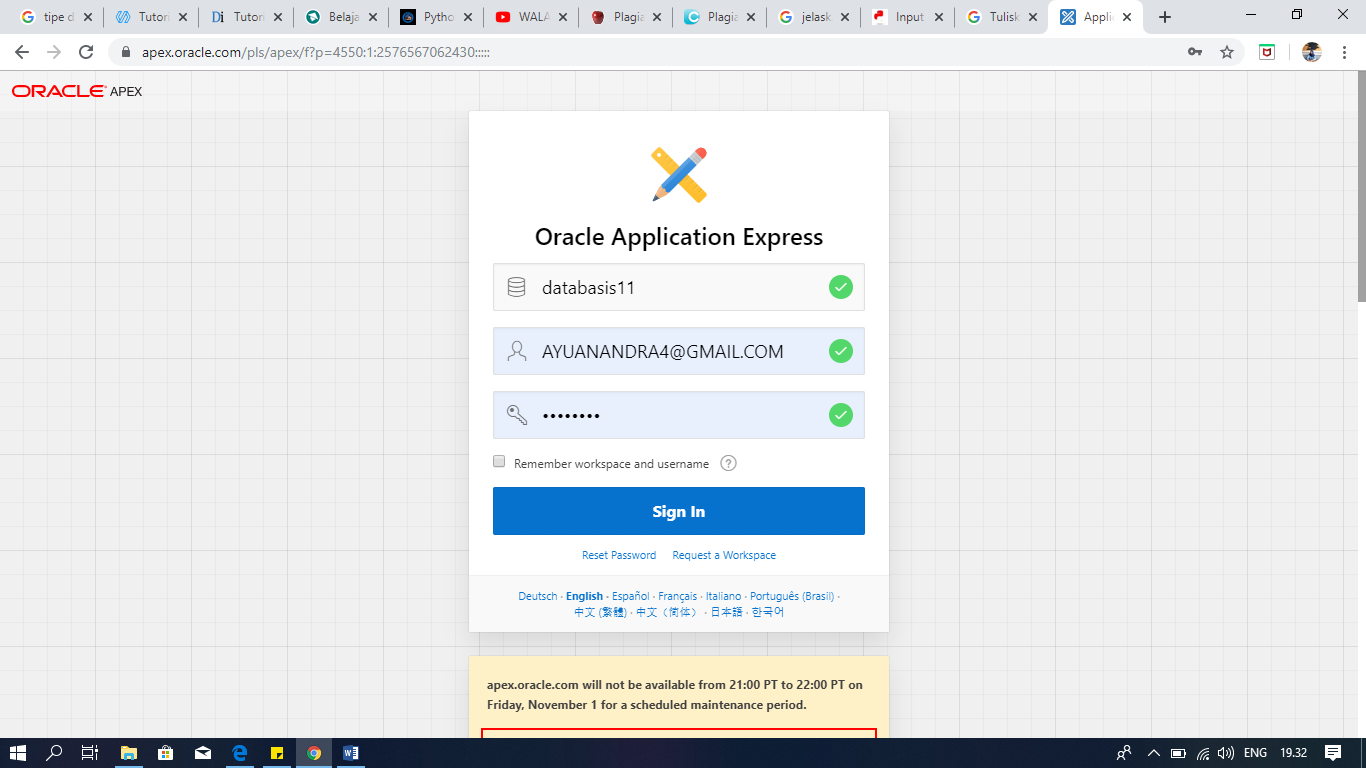
\includegraphics[width=11cm\textwidth]{Untitled0.png}
\end{center}

\section{Pilih App Builder Untuk Membuat Aplikasi}
\begin{center}
    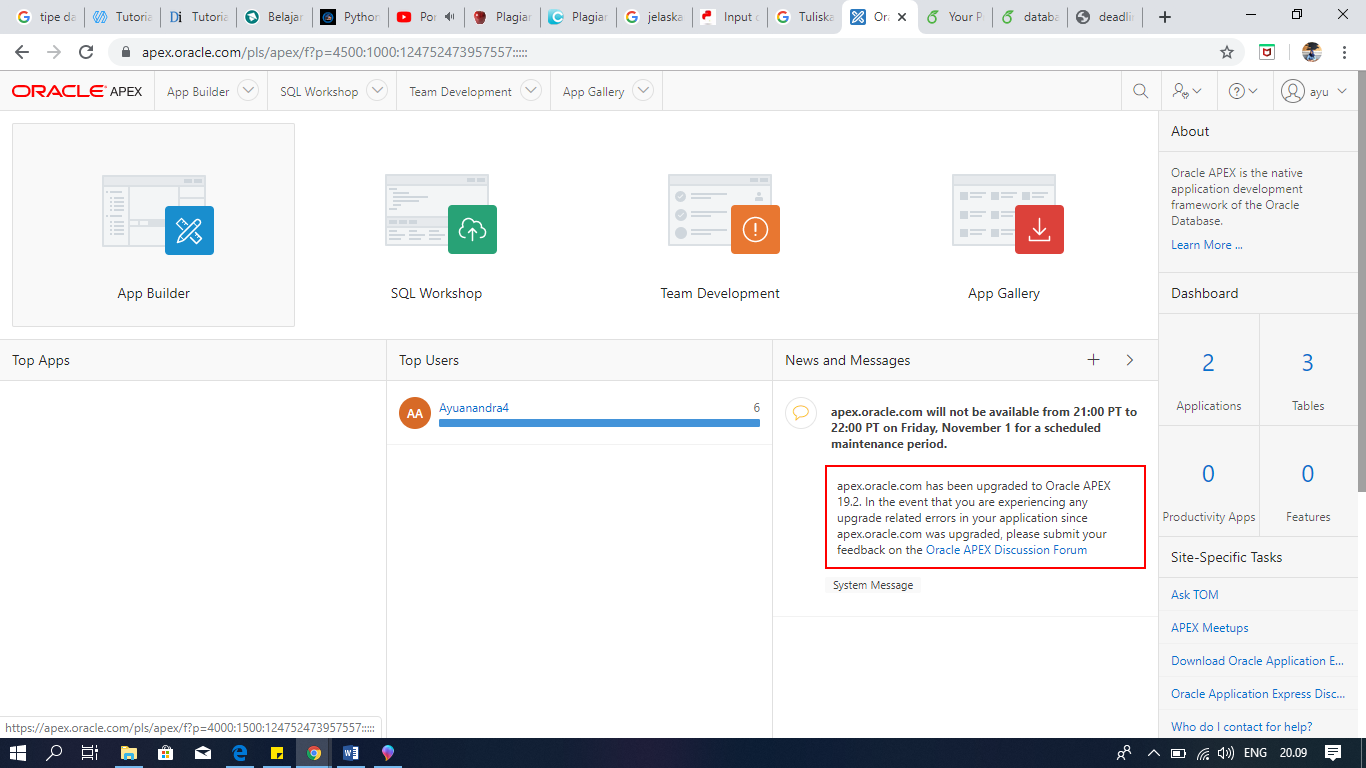
\includegraphics[width=11cm\textwidth]{app.png}
\end{center}

\section{Pilih create}
\begin{center}
    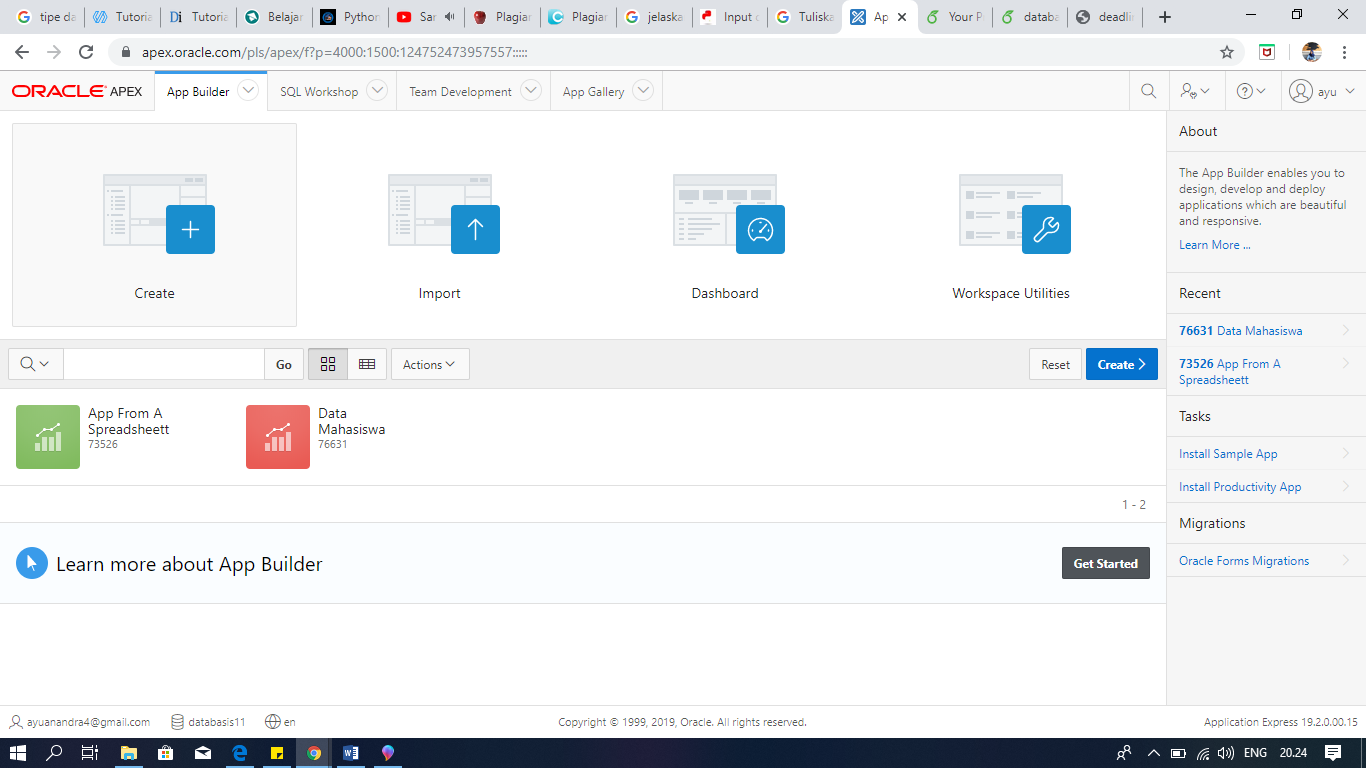
\includegraphics[width=11cm\textwidth]{create.png}
\end{center}

\section{Pilih From a File untuk memasukan data}
\begin{center}
    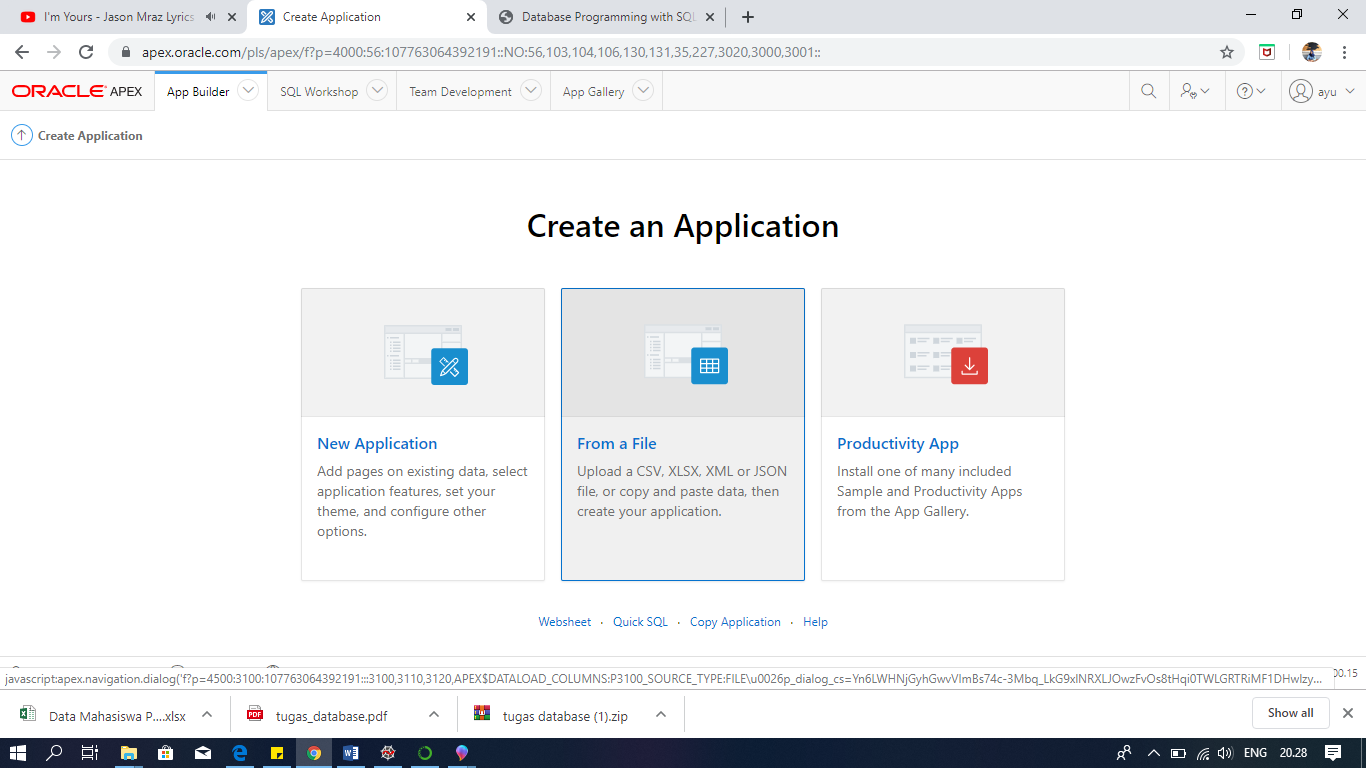
\includegraphics[width=11cm\textwidth]{Untitled.png}
\end{center}

\section{Memasukan File, Pilih Dari Laptop Masing-Masing}
\begin{center}
    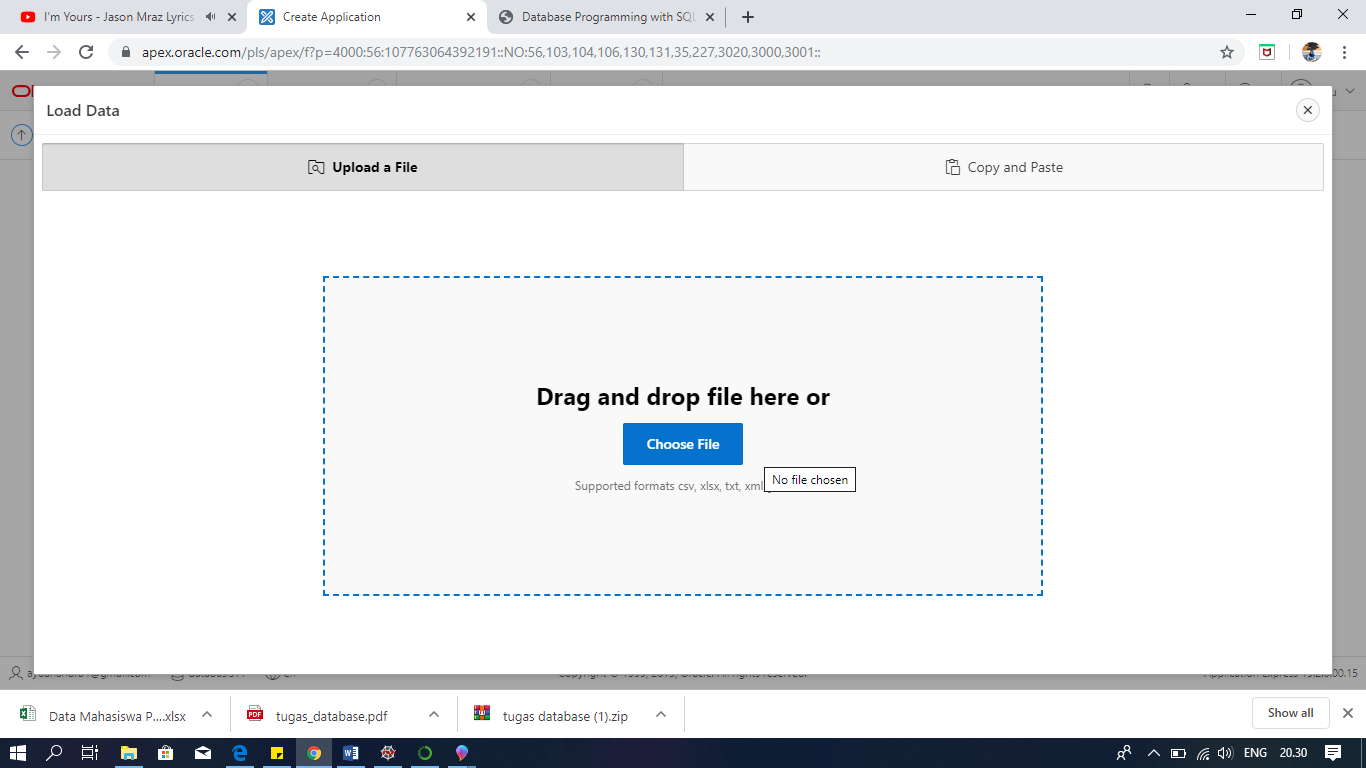
\includegraphics[width=11cm\textwidth]{Untitled1.png}
\end{center}

\section{Mengisi Nama Data Table}
\begin{center}
    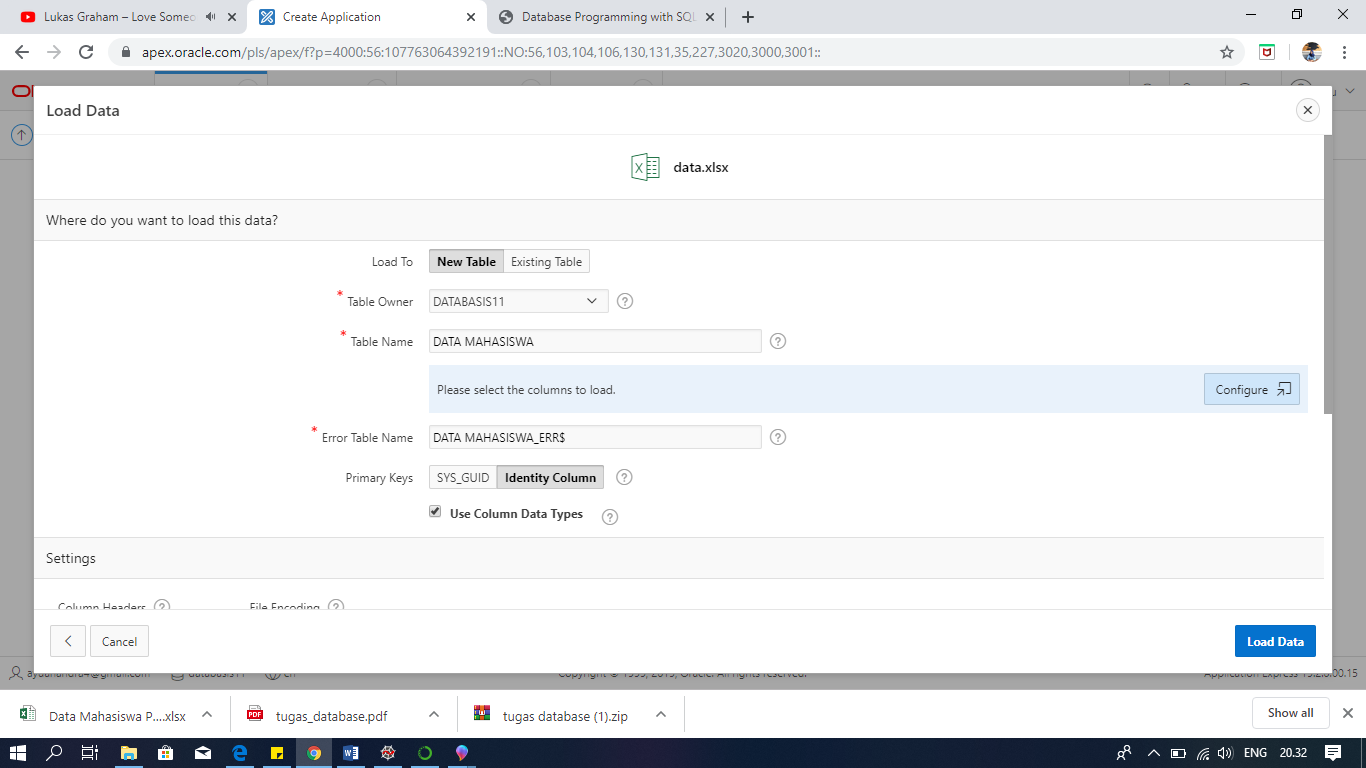
\includegraphics[width=11cm\textwidth]{Untitled2.png}
\end{center}

\section{Setelah Load Data, Data Berhasil Di Inputkan}
\begin{center}
    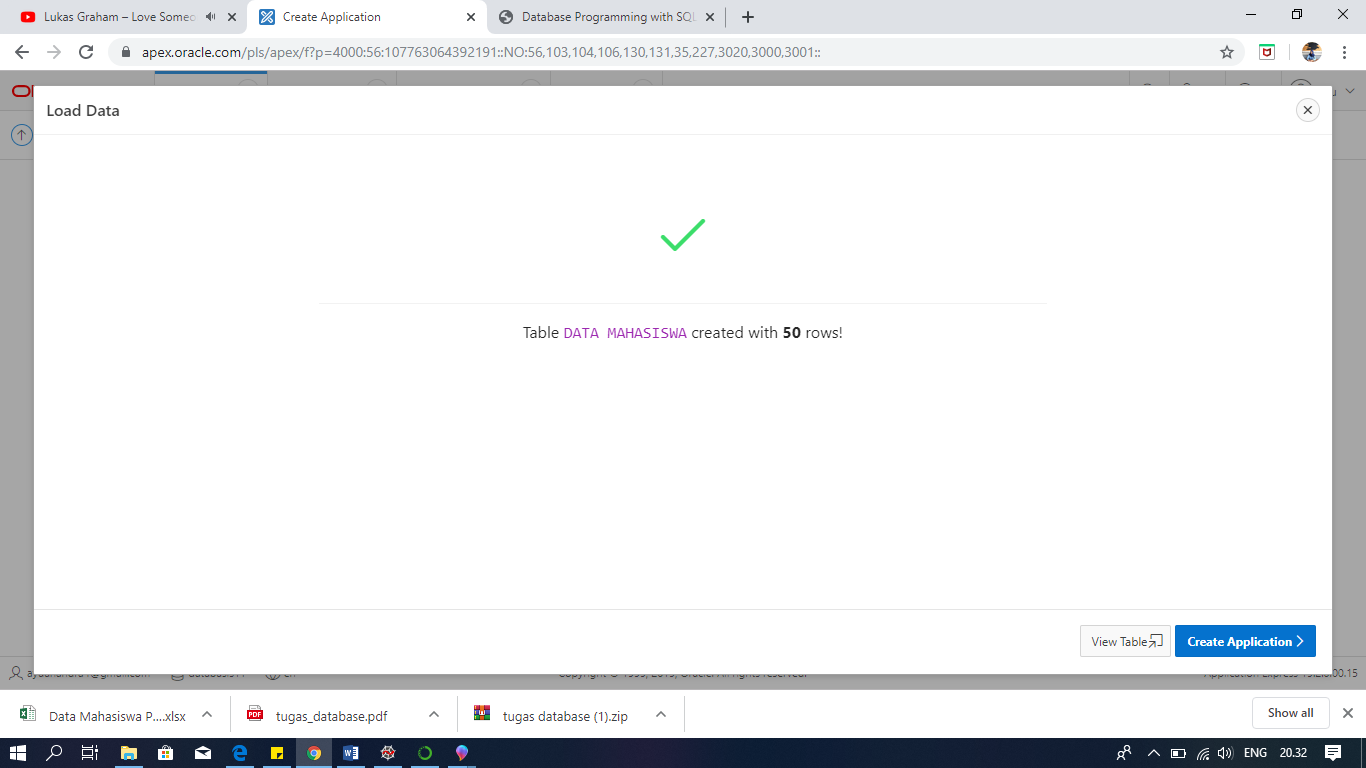
\includegraphics[width=11cm\textwidth]{Untitled3.png}
\end{center}

\section{Lalu Check All, Features}
\begin{center}
    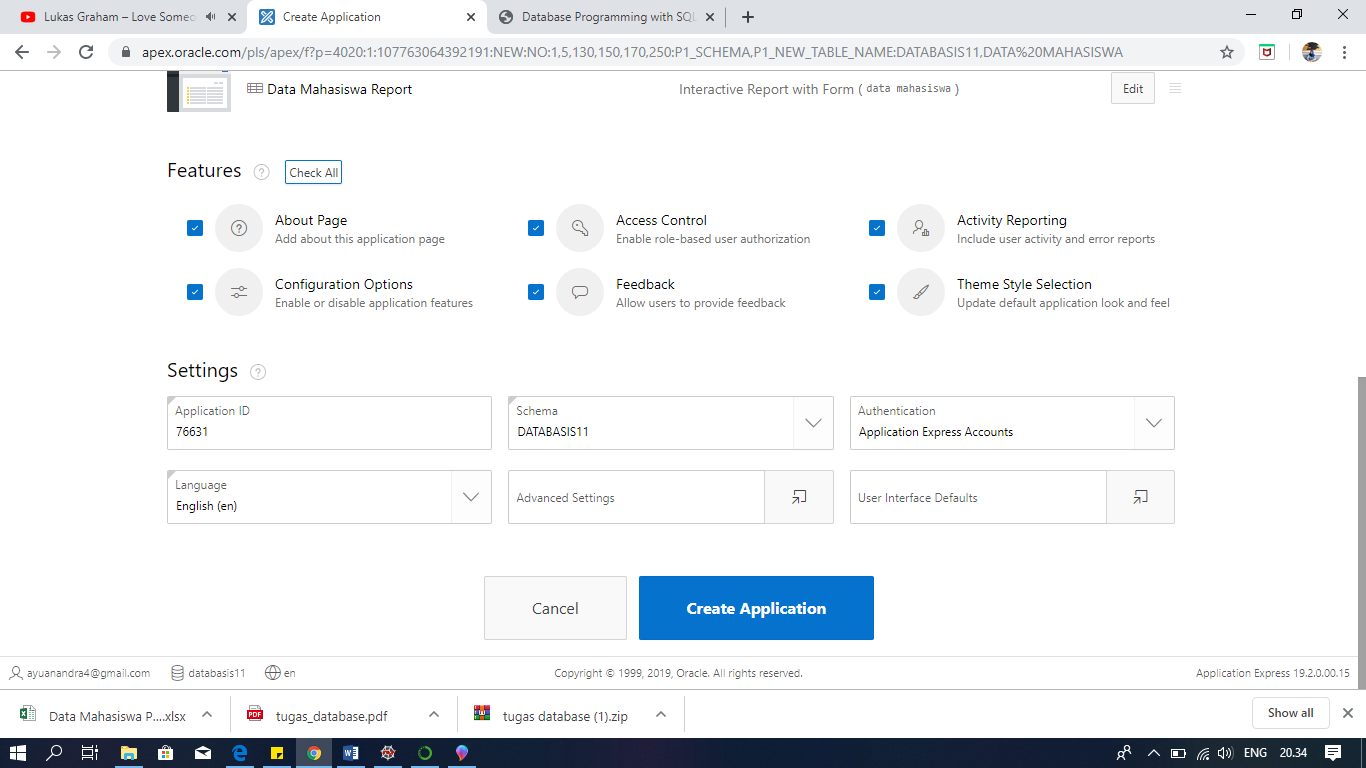
\includegraphics[width=11cm\textwidth]{Untitled4.png}
\end{center}

\section{Kemudian dapat Langsung Run Aplikasi}
\begin{center}
    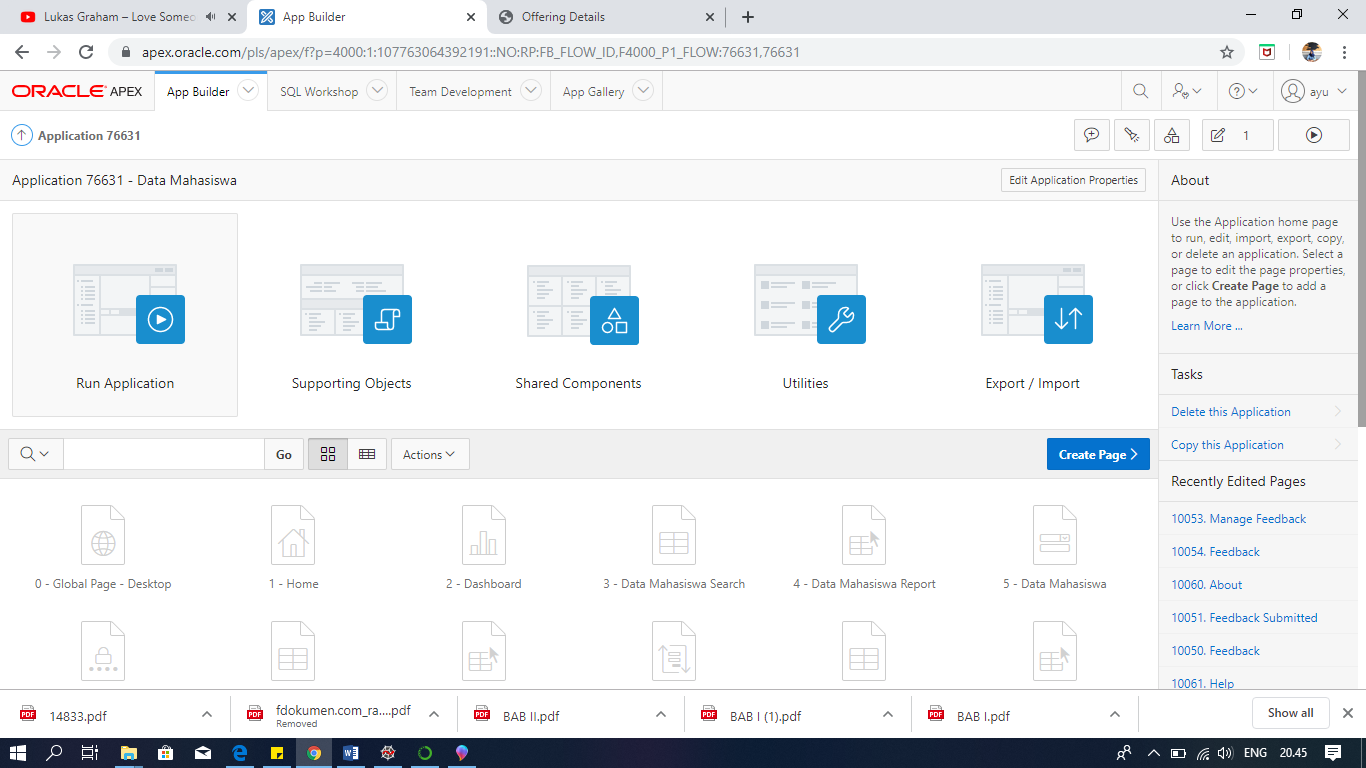
\includegraphics[width=11cm\textwidth]{Untitled5.png}
\end{center}

\section{Aplikasi nya telah Terbuat}
\begin{center}
    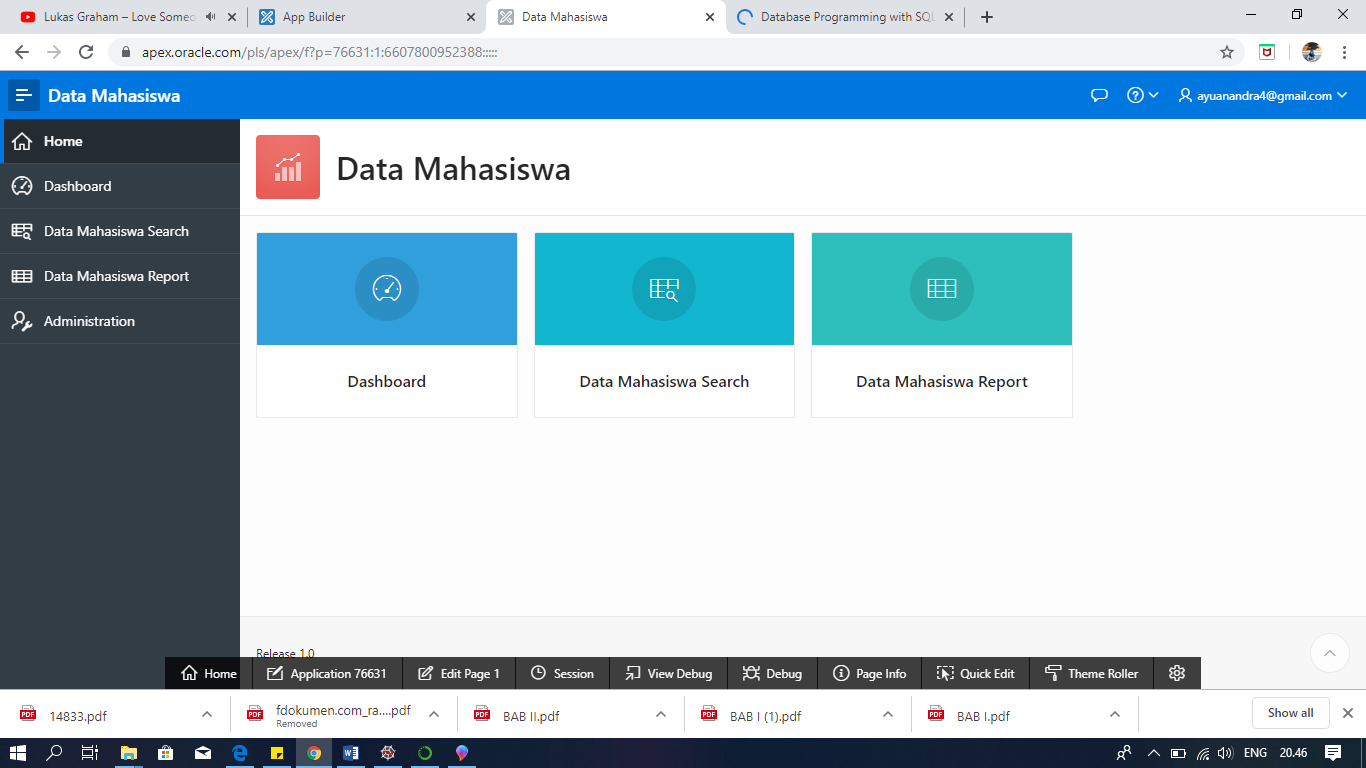
\includegraphics[width=11cm\textwidth]{Untitled6.png}
\end{center}

Workspace : databasis11
Username : AYUANANDRA4@GMAIL.COM
Password : anandra4

\end{document}

